\endnote{\glqq Diagramm einer Schwingung\grqq{} von Till Blaha - Eigenes Werk. Lizenziert unter Gemeinfrei.}

\begin{figure}[h!]
	\centering
	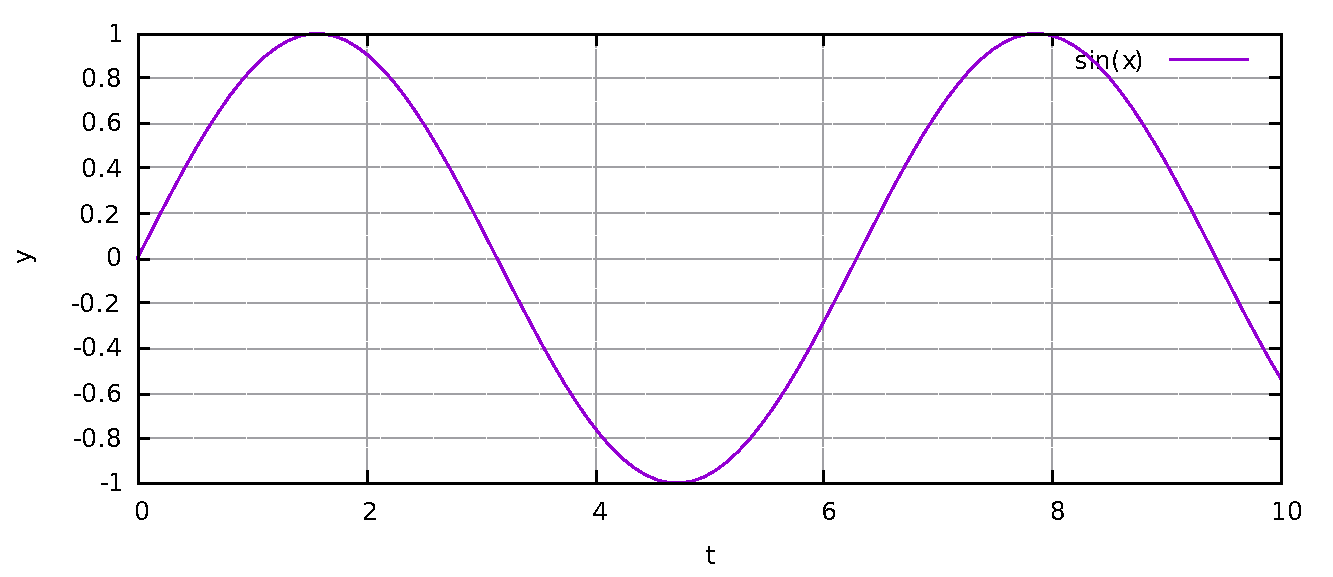
\includegraphics[width=0.9\textwidth]{schwingung}
	\begin{comment} 'plot_pitics.p'
set dummy t
set ylabel "s"
set xlabel "t"
set output 'schwingung.png'
plot sin(t) ls 1 title 's(t)=sin(t)'
	\end{comment}
	\caption{Diagramm einer Schwingung: Elongation über der Zeit}
\end{figure}

